%%%%%%%%%%%%%%%%%%%%%%%%%%%%%%%%%%%%%%%%%%%%%%%%%%%%%%%%%%%%%%%%%
%
% Project     : Bachelorarbeit
% Title       : Machbarkeitsanalyse für eine ressourcenorientierte Schnittstelle zur Verarbeitung grundlegender Probleme der Informatik
% File        : fazit.tex Rev. 01
% Date        : 01.03.2015
% Author      : Raffael Santschi
%
%%%%%%%%%%%%%%%%%%%%%%%%%%%%%%%%%%%%%%%%%%%%%%%%%%%%%%%%%%%%%%%%%


\chapter{Schlussfolgerungen}\label{chap.Schlussfolgerungen}
In diesem Kapitel wird kurz auf den ersten Einsatz des Produkts, das Fazit des Verfassers und den Ausblick der Schnittstelle eingegangen.

\section{Verwendung}\label{fazit_verwendung}
Während der Projektzeit konnte der Spielplan des Auffahrtsturniers des Turnvereins Grafstals validiert werden. Dieser Spielplan wird von Hand erstellt. Dabei unterlaufen immer wieder 
kleine Patzer, was bei einer Planung von etwa 110 Spielen und Schiedsrichtern, welche zudem Coaches für bis zu drei Teams sind, nicht verwunderlich ist. Diese Aufgabe hat zum einen die Schnittstelle 
getestet, hat jedoch auch dem Verein geholfen, da auch dieses Jahr zwei kleine Fehler auftauchten. Der Turnverein hat sich bereits sehr für die vollautomatische Lösung interessiert.

\section{Fazit}\label{fazit}

Das Erstellen eines Konzepts einer solchen Schnittstelle stellte sich als sehr spannend heraus. Die Recherche und die Analyse der Probleme mit hoher Laufzeitkomplexität war sehr fesselnd und es 
bestand die Gefahr, sich darin zu verlieren. Das Gebiet der theoretischen Informatik ist extrem weitreichend und die Probleme können beliebig komplex werden. Es war schnell klar, dass es schwierig 
sein wird, eine generische Lösung für alle Probleme zu finden. Das Konzept mit dem pre- und post-Aktionen ist jedoch eine elegante Lösung, welche sehr viel Flexibilität bietet. Der Ablauf einer Berechnung 
konnte generisch gehalten werden und somit ist die Machbarkeitsstudie als erfolgreich zu betrachten.

Die Auswahl der Probleme hat sich als facettenreich herausgestellt und das Auswahlverfahren hat sich bewährt. Es ist spannend, dass die beiden Probleme aus dem Bereich `Netzwerk Design' 
viele Ähnlichkeiten aufzeigen, jedoch mit komplett anderen Algorithmen gelöst werden. Die beiden Planungsprobleme sind sich sehr ähnlich und könnten ziemlich sicher mit einem generischen 
Algorithmus gelöst werden. Der grösste Unterschied liegt darin, dass bei einem Spielplan zwei Mannschaften gleichzeitig auf einem Platz sind, bei einem 
Stundenplan jedoch nur eine Klasse im Klassenzimmer ist. Der Code der Schnittstelle konnte für die beiden Planungsprobleme auch viel generischer gehalten werden als für diejenigen aus dem Bereich 
`Netzwerk Design'.

Der Entscheid, eine dokumentorientierte Datenbank zu verwenden, war ideal. Die Flexibilität der Datenbank kam dem Projekt sehr zugute und es wurden auch keine bekannten Funktion von relationalen 
Datenbanken vermisst. Spring Boot ist für einen Prototyp ideal, da es schon sehr viel mitbringt. Dies kann jedoch auch zu Problemen führen, da die Versionen der Libraries nicht selber verwaltet 
werden können. 

Ich bin mit dem Konzept und dem entstanden Prototypen sehr zufrieden und freue mich nun auf die Planung der nächsten Schritte. Mit Spannung erwarte ich die ersten realen Kunden, welche diese 
Schnittstelle verwenden und ich bin gespannt, wohin sich dieses Projekt entwickeln wird. Ich bin mir bewusst, dass die Schnittstelle noch keine Produktionsreife hat. Es benötigt jedoch nicht mehr viel bis die 
ersten Turnierpläne vollautomatisch erstellt werden können.

\section{Ausblick}\label{fazit_ausblick}

Das Konzept ist nun ausgearbeitet, jetzt wird eine automatisierte Lösung angestrebt. Als nächstes wird die Integration von zwei Teilprojekten geplant. Dabei handelt es sich um die Entwicklung eines 
Verarbeitungssystems mit einer eigenen Cloud Lösung und um die Ansteuerung eines generischen Planungsalgorithmus. Danach wird es weiteren Entwicklungsaufwand geben, da eine 
Webseite für die Eingabe für Kleinkunden angedacht ist. Da die Endlösung schliesslich dem Nutzer eine ungefähre Berechnungszeit angeben möchte, wird zusätzlich eine Berechnungskomponente 
benötigt. Diese Komponente wird wahrscheinlich mittels Heuristiken und alten Resultaten eine Zeitextrapolation erstellen. Der Grundstein für diese Berechnung ist mit dem vorgestellten Konzept 
bereits gelegt, da die Zwischenresultate und Endresultate einen Zeitstempel enthalten. Dadurch kann berechnet werden, wie lange die Berechnung zu einem gewissen Resultat gedauert hat. In 
\autoref{fig:ausblick} ist das Konzept des übergeordneten Projekts dargestellt, von welchem Teile des User API und der Data Controllers in diesem Projekt behandelt wurden.

\begin{figure}[h]
\centering
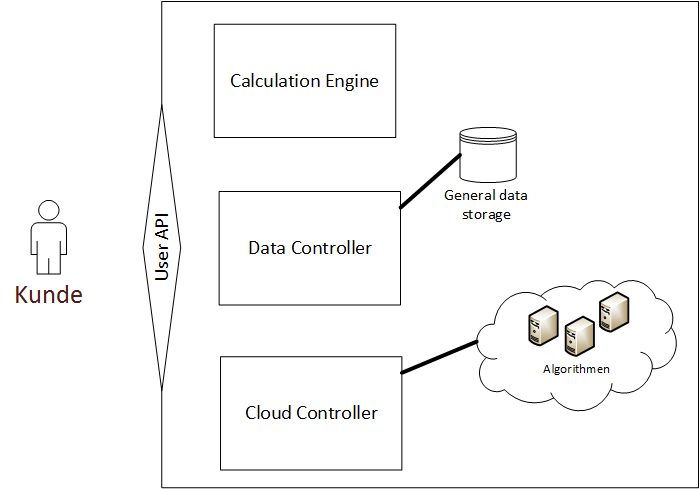
\includegraphics[scale=0.8]{images/visio/ausblick.png}
\caption[Konzept des übergeordneten Projekts]{Konzept des übergeordneten Projekts \selfmade{}}
\label{fig:ausblick}
\end{figure}